\documentclass[a4paper]{article}

\usepackage{numprint}
\usepackage{nameref}
\usepackage{float}
\usepackage{url}
\usepackage{graphicx}	% For figure environment
\usepackage{epstopdf}
\usepackage[center]{subfigure}
\usepackage{amssymb}	% For mathematical figures like \mathbb{R}
\usepackage{amsmath}
\usepackage{framed}
\usepackage{tikz}
\usetikzlibrary{mindmap,trees}
\usepackage{pdflscape}
\usepackage[a4paper]{geometry}
\usepackage{subfiles}
\usepackage{listings}
\usepackage{color}

\definecolor{dkgreen}{rgb}{0,0.6,0}
\definecolor{gray}{rgb}{0.5,0.5,0.5}
\usepackage{array}
\usepackage{booktabs}% http://ctan.org/pkg/booktabs
\usepackage{xparse}% http://ctan.org/pkg/xparse
% Rotation: \rot[<angle>][<width>]{<stuff>}
\NewDocumentCommand{\rot}{O{45} O{1em} m}{\makebox[#2][l]{\rotatebox{#1}{#3}}}%
\definecolor{mauve}{rgb}{0.58,0,0.82}

\lstset{frame=tb,
  language=Java,
  aboveskip=3mm,
  belowskip=3mm,
  showstringspaces=false,
  columns=flexible,
  basicstyle={\small\ttfamily},
  numbers=none,
  numberstyle=\tiny\color{gray},
  keywordstyle=\color{blue},
  commentstyle=\color{dkgreen},
  stringstyle=\color{mauve},
  breaklines=true,
  breakatwhitespace=true
  tabsize=3
}


\title{Advanced Systems Lab - Milestone II} 
\author{Lukas Elmer (elmerl@ethz.ch)} 
\date{\today} 


\begin{document}

\maketitle

\pagebreak

\tableofcontents

\pagebreak

\begin{abstract}

This document is the follow up document of Advanced Systems Lab - Milestone I and describes an analytical queueing model of the system which was built using the operational laws. Using this model, the performance characteristics of the model are derived and compared to the measurements of Milestone I. Furthermore it is analysed where the data matches the model and where it does not.

\end{abstract}

\pagebreak

%% ----------------------------------------------
% Section Messaging System
%% ----------------------------------------------
\section{Tasks}

* analytical queuing model
** for each component of the system
** and for the system as a whole.

* derive the performance characteristics that the model predicts
** compare them with the results obtained in milestone 2

* Explain where the model and data match and where they do not match
** sufficiently detailed explanations of characteristics behind the observed behaviour
*** code
*** system
*** hardware

* the modeling should include for each component
** the queuing model(s)
** parameters

* overall system should be modeled
** as queuing network
** the experimental results analyzed using the operational laws

* clearly indicate
** the behavior expected from the model through graphs
** plot them together with the measured behavior

* When evaluating the experimental data and the models
** clearly indicate the laws you are applying
** explain why you think they can be applied in the corresponding analysis


\section{Introduction}

\subsection{Data Sources}

This document extends the document of milestone I. Especially the following test runs are used in this analysis:

\begin{itemize}
\item Microbenchmarks
\item 2 hour test
\item Scaleout experiments
\end{itemize}

\subsubsection{Scaleout Experiments}

Some additional scaleout experiments were conducted. They were executed with 4 middlewares distributed on 2 virtual machines. For the client and middleware instances, Amazon instances of the type m1.small was used, and for the database the type m1.medium was used.\\
\noindent Then, the number of clients was scaled from in steps of 15 from 15-60, and in steps of 30 from 60-300.


%% ----------------------------------------------
\section{Components}

In the analysis, the focus of the system is on the middleware. Additionally, the database is modelled as a queue, but no further internals of the database are considered.\\

\begin{figure}[H]
	\begin{center}
    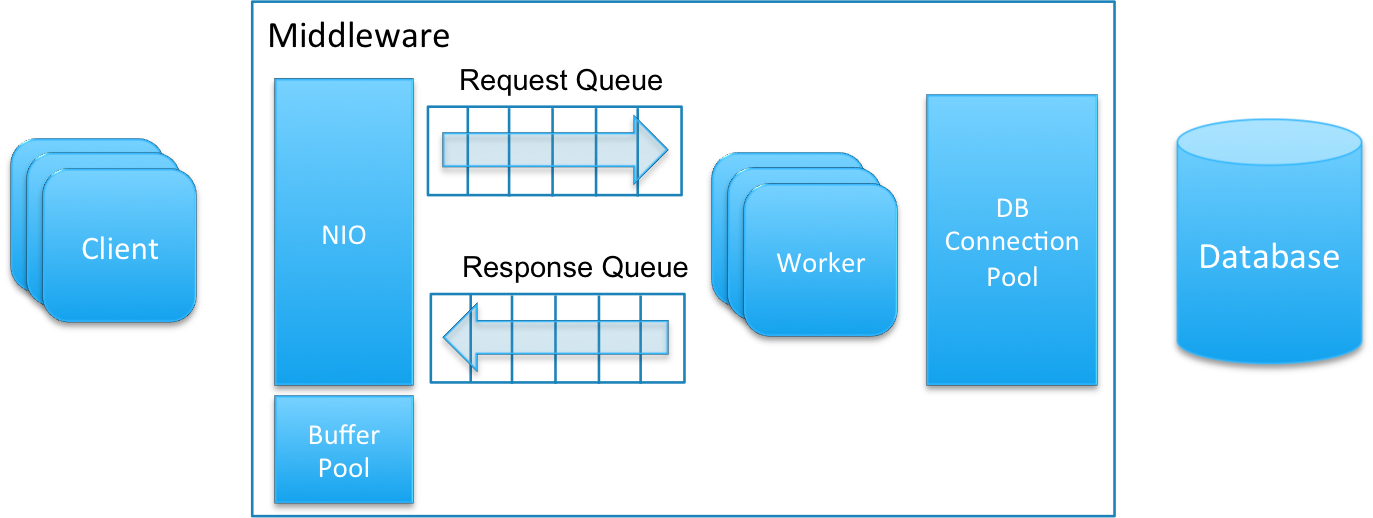
\includegraphics[scale=0.6]{../drawings/broker-threading.png}
  \end{center}
  \caption{Middleware's main Components}
  \label{fig:middleware-threading}
\end{figure}

Figure \ref{fig:middleware-threading} shows a overview of the systems components. The most important parts of the analytical models are:

\begin{itemize}
\item The middleware (multiple instances)
	\begin{itemize}
	\item NIO (network input and output, single queue)
	\item Request queue (when the requests are waiting for workers)
	\end{itemize}
\item The database (modelled as a single queue)
\end{itemize}

Because the clients wait for the current message to be answered before sending the next message, the system is modelled as a \textbf{closed system}. If messages fail to be processed by the middleware, the client implements a backoff time, so the system doesn't get overloaded.

\section{Performance Characteristics}

As described in the book (TODO) in section 30.1, a queuing system can be specified by six parameters. Therefore we use the Kendall notation in the form A/S/m/B/K/SD, where the letters correspond to the six parameters listed on page 507-509 in the book. Unless specified otherwise, when A/S/m is written, then this corresponds to a A/S/m/$\infty$/$\infty$/FCFS queue, where FCFS means First Come First Serve\footnote{https://en.wikipedia.org/wiki/First-come,\_first-served}.

\subsection{A: Arrival Process}

Even tough the clients send in a certain deterministic interval, because of the network and the operating system there is a delay until the requests arrive in the queuing system. We assume that this delay is exponentially distributed. Thus, A is the Markovian M. (can be seen in figure TODO)

\subsection{S: Service Time Distribution}

The service time distribution also is assumed to be distributed exponentially. We also know that the service time is memoryless - i.e. it does not matter what request happened before the current request. This can be assumed because there is no caching implemented.

\subsection{m: Number of Servers}

The number of servers is the amount of middlewares running.

\subsection{B: System Capacity}

The system capacity is defined by those who are waiting for service and those who receive service.  This is dependent on how many requests a middleware can accept. Because there are always less clients connected to a middleware then connections to the NIO part of the middlware can be established, the system capacity will be the same as the population size.\\

Unless otherwise specified, 

\subsection{K: Population Size}

The population size is defined by the amount of clients issuing requests to the middleware.

\subsection{SD: Service Discipline}

In general, the service discipline is First Come, First Served (FCFS). However, because there are limited CPU's on the middleware, and CPU's usually use Round Robin (RR), this may have to be considered in the analysis.


\section{Model}

\subsection{General Model}

The following queueing model network was created based on the understanding of the closed system as shown in figure \ref{fig:general-queueing-network}.

\begin{figure}[H]
	\begin{center}
    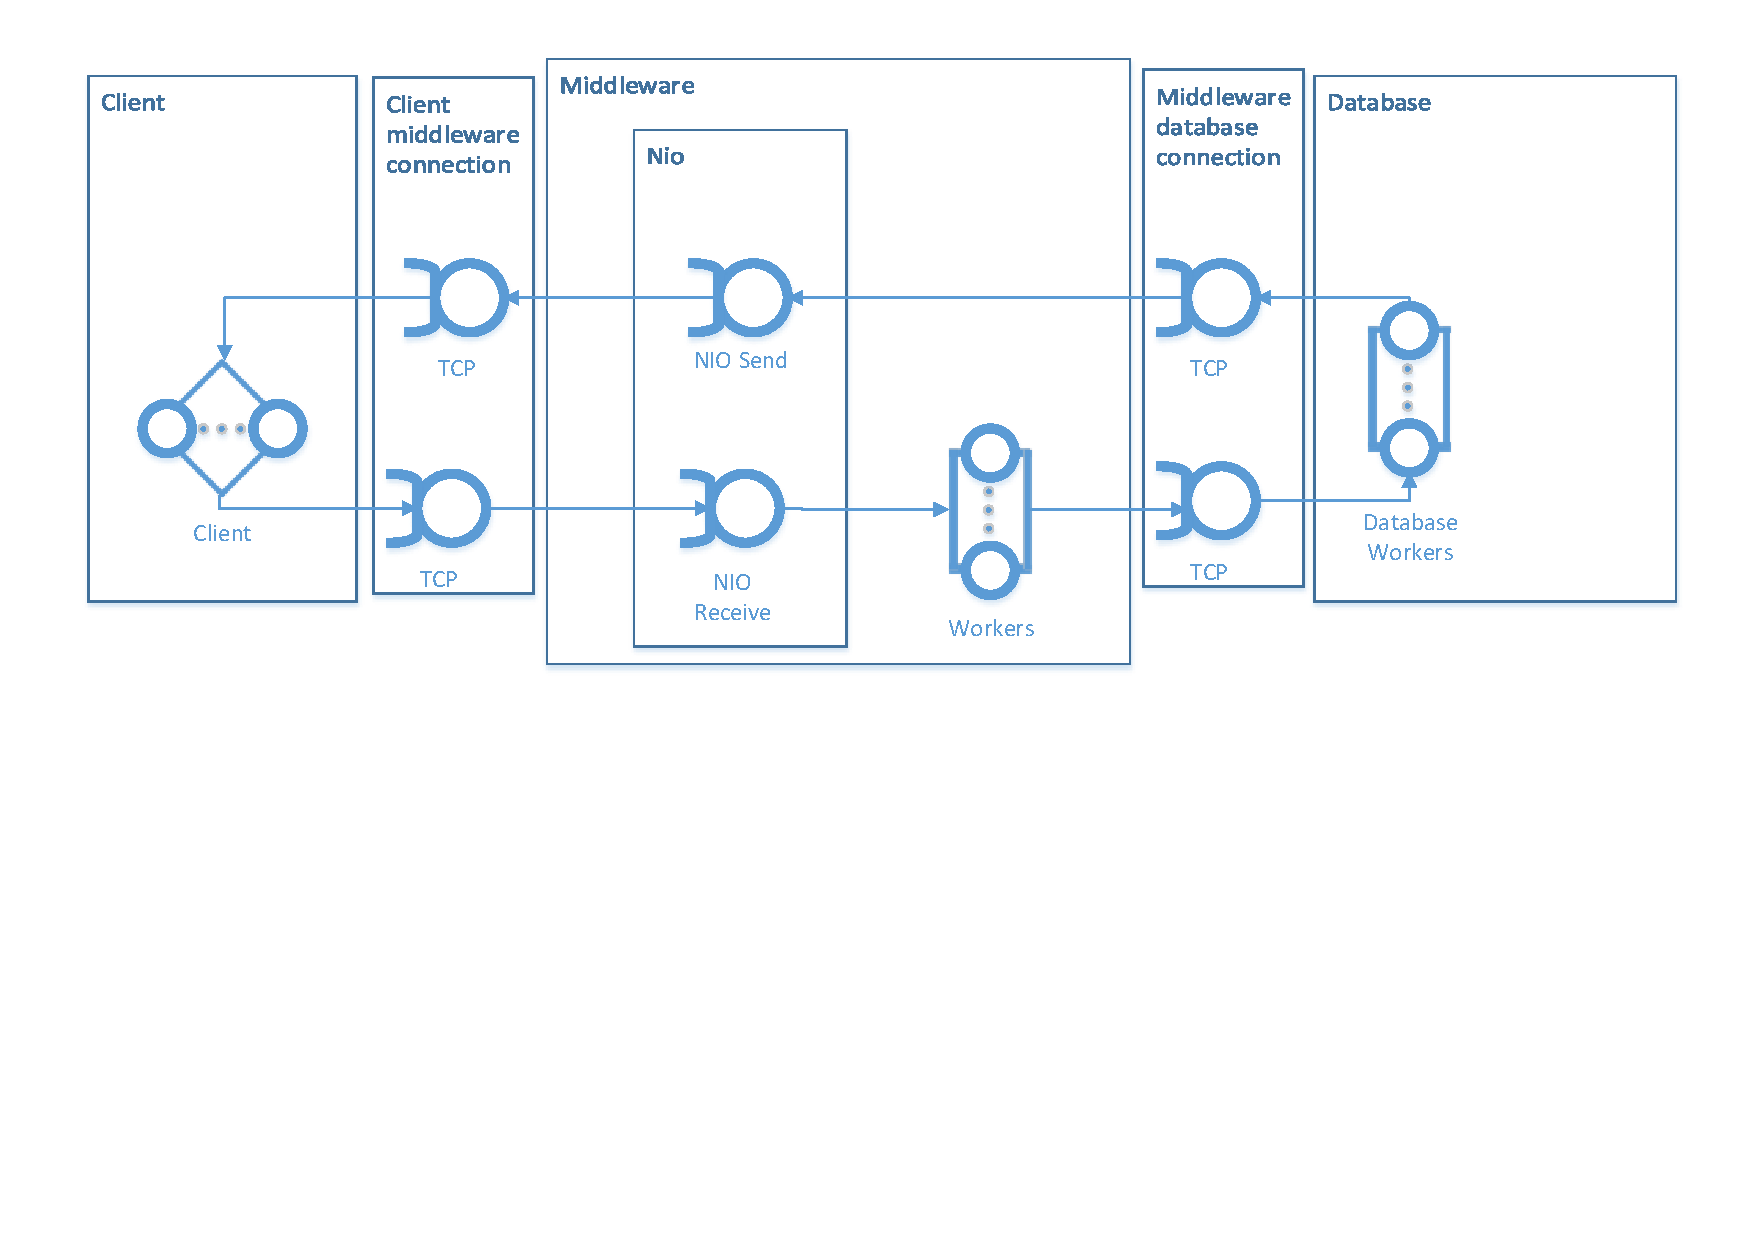
\includegraphics[scale=0.6, trim = 15mm 94mm 12mm 10mm, clip]{../drawings-ms2le/general-queueing-network.pdf}
  \end{center}
  \caption{general queueing network}
  \label{fig:general-queueing-network}
\end{figure}


\subsection{Simplified Model}

\noindent Initially the TCP connections are modelled as a separate System. To be precise, these TCP connections would influence one another. In the simplified model, those TCP connections act as separate queues. Additionally, the NIO part of the middleware is included in the TCP connection queue. This is a good idea because the NIO thread and the network are strongly linked and the NIO processing is very fast.\\

\noindent Next, the model was further simplified by separating the NIO component into two separate queues. In the real system however, similar to the TCP connection, there is only one NIO thread.\\

\noindent Furthermore, the TCP network connection between the middleware and the database is separated. In the real system, this would be the same connection.\\

\noindent To further simplify the model, the TCP connections are modeled as delay centers instead of queues. This should be ok, because the network connection utilization is not at it's limit during the test runs.\\

\noindent Those simplifications then lead to the simplified queueing network as shown in figure \ref{fig:simplified-queueing-network}. Note that the TCP connections are still drawn as queues, but they are modeled as delay centers instead.\\


\begin{figure}[H]
	\begin{center}
    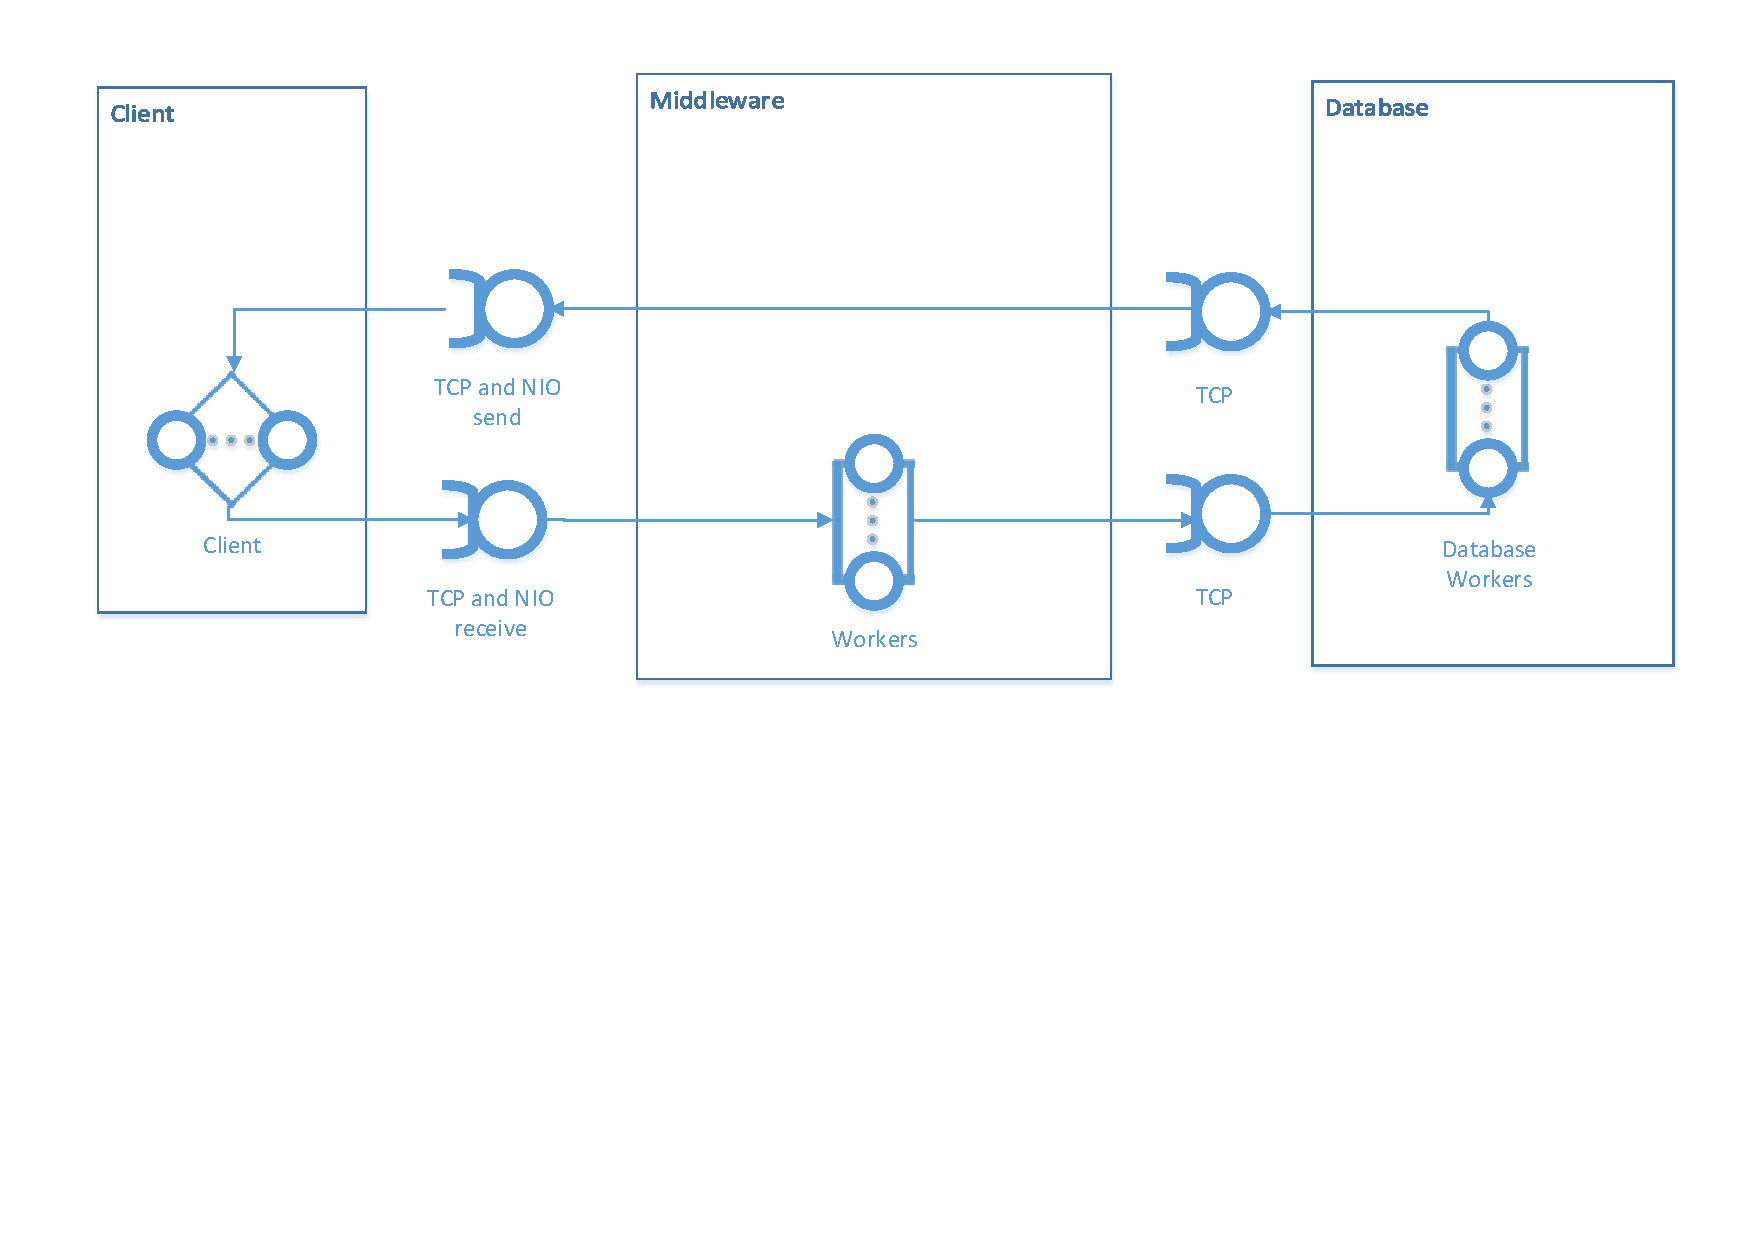
\includegraphics[scale=0.6, trim = 15mm 94mm 12mm 10mm, clip]{../drawings-ms2le/simplified-queueing-network.pdf}
  \end{center}
  \caption{simplified queueing network}
  \label{fig:simplified-queueing-network}
\end{figure}

\subsection{Service Centers}

\subsubsection{Client: M/M/$\infty$/$\infty$/$\infty$/FCFS}

The clients do simple operations (send and receive messages) and don't do any computation. The think time (\textbf{Z}) of the client doesn't depend on the client count and thus correspond to the sleep time between requests.\\

\noindent The think time of the clients is 10ms.\\

For the scaleout test, the number of clients was scaled from 15, 30, 45, 60.

\subsubsection{TCP and NIO receive / send: M/M/$\infty$/$\infty$/$\infty$/FCFS}

The TCP and NIO receive / send contains many things like the network card, the time it takes to physically transport and rout the signal to the corresponding receiver, the OS buffer, and the JVM network buffer. It was decided to also add the NIO thread to this queue, because it acts like the OS buffer or the JVM network buffer.\\

\noindent According to the Java specification, the buffer of the TCP connection is 50, and thus the queue should be modeled as M/M/$\infty$/50/$\infty$/FCFS. However, to simplify the model, it is modeled as M/M/$\infty$/$\infty$/$\infty$/FCFS.\\

\noindent The queue is modelled as a fixed capacity service center with and unbound queue size. Because only one network connection and one NIO thread is used, the service node count is 1. So it is modelled as M/M/$\infty$/$\infty$/$\infty$/FCFS queue.\\

\noindent In the following analysis, the "TCP and NIO receive" and the "TCP" are merged together as TCP.

\noindent Another thing that could have been modelled would have been the separation of sending and receiving messages. For this, the database would be split up into two parts, one for sending and one for receiving respectively. However, to keep the model simple, this hasn't been done.


\subsubsection{TCP M/M/$\infty$/$\infty$/$\infty$/FCFS}

This is the same as \textbf{TCP and NIO receive} without the NIO. Therefore it is also modelled as a fixed capacity service center with unbound queue size and a node count of 1.\\

\noindent As measured in the milestone I, the mean service time of the TCP connection is 2.644ms for sending and 2.590ms for receiving messges. For this analysis, the mean of 2.617ms is assumed to simplify the analysis.\\

\noindent In the following analysis, the "TCP and NIO receive" and the "TCP" are merged together as TCP.


\subsubsection{Workers (Middleware): 80 * M/M/1/$\infty$/$\infty$/FCFS}

There are several worker threads in the system. These worker threads are modelled as a M/M/x queue, where x corresponds to the number of worker threads per middleware. The workers obviously are load dependent. The queue size is 100, as it corresponds to the queue size of the queue from which the worker threads can get the requests which have to be processed.\\

\noindent Additionally, the middlewares can be scaled. The clients are evenly distributed between the middlewares, and so are the requests sent by the clients. Therefore, the model is simplified further as follows: for every additional middleware, the workers are merged into one big worker pool across all middlewares. Therefore, the middleware queues are modelled as (n * x) * M/M/1/$\infty$/$\infty$/FCFS queues, where n corresponds to the amount of middlewares and x corresponds to the number of worker threads per middleware.\\

For the scaleout test, 4 middlewares were used, each with 20 workerthreads. This gives a total of 4*20 = 80. The visit count for the middleware is 1/80, because one messages passes through exactly one middleware worker.\\

The service time of the middleware is calculated as follows:
Total service time - DB service time - 4 * TCP service time. As estimated in the milestone I, for sending the service time is 0.042ms and for receiving it is 0.043ms. For the analysis, a service time of 0.042ms is used.\\


\subsubsection{Database M/M/8/$\infty$/$\infty$/FCFS}

As stated in the requirements, there must be only one database. However there is never a global table lock and there are multiple ECU's (EC2 Compute Unit\footnote{https://aws.amazon.com/en/ec2/faqs/\#What\_is\_an\_EC2\_Compute\_Unit\_and\_why\_did\_you\_introduce\_it})  available. Furthermore it's unknown how the hardware of the Amazon medium instance is exactly built, but it can be considered that it takes advantage of advanced technology like the locality effect, caching, fail-safe and performance optimized hardware. Unfortunately in one hand, fortunately in the other hand, details about the hardware which the system runs on is unknown. Further information can be found on the amazon website\footnote{https://aws.amazon.com/en/ec2/instance-types/}.\\

Even tough there are 2 ECU's: because there is one vCPU for the medium instance, the node count was first set to 1. Unfortunately this yielded bad results. Therefore, multiple values for the node count were tested. The best results were achieved with a node count of 8. One reason to explain this may be that the database implements bulk IO operations and stores the corresponding pages in the cache. Also, the vCPU instance implements hyperthreading, so more vCPU power is available than only one vCPU.\\

The service center is modelled as load dependent for obvious reasons.\\

The service time is 4.016ms for sending and 6.196ms for receiving messages, as measured in the microbenchmarks. For this analysis, the mean of 5106ms was used first. Unfortunately, because sending a message is faster then receiving a message, there are more messages sent then received. Therefore the service time for the database had to be adjusted to 4.506ms.\\

\section{Mean Value Analysis}

The mean value analysis is performed as described in the book used in this course\footnote{The Art of Computer Systems Performance Analysis, Raj Jain, 1991}. Here, the values of the microbenchmarks of milestone I are used:

\noindent The mean value analysis is based on the scaleout experiment conducted during this milestone.\\


%\noindent To calculate the mean arrival time and the mean service rate, the scaleout experiment with 60 clients was used. This gives a mean arrival rate ($\lambda$) 178.885 messages per second. The mean service time for this test was 32.99374762ms, and there are 80 workers, which gives a mean service rate of 1 / 32.99374762ms / 80 workers = 0.37885966 requests/s/worker and 30.30877278 requests/s in total. \\


\noindent The number of clients varies from 15-300\footnote{from 15-60 in steps of 15, from 60-300 in steps of 30}.\\


\begin{tabular}{|l|l|r|r|r|}
\hline
\textbf{Variable} & \textbf{Description} & \textbf{Value} \\ \hline
$N_{client}$ & \# clients & 15-300 \\ \hline
Z & client think time & 10ms \\ \hline
$N_{middleware}$ & \# middleware workers & 80 \\ \hline
$S_{middleware}$ & middleware service time & 0.042ms \\ \hline
$V_{middleware}$ & middleware visit count & 1/80 \\ \hline
$N_{tcp}$ & \# TCP & 80 \\ \hline
$S_{tcp}$ & TCP service time & 2.617ms \\ \hline
$V_{tcp}$ & TCP visit count & 4 \\ \hline
$N_{db}$ & \# DB Workers & 8 \\ \hline
$S_{db}$ & DB service time & 5.106ms \\ \hline
$S_{db}$ & DB service time (fixed version) & 4.506ms \\ \hline
$V_{db}$ & DB visit count & 1 \\ \hline
\end{tabular}
\\

\subsection{Results}

\begin{landscape}\begin{figure}[H]
	\begin{center}
    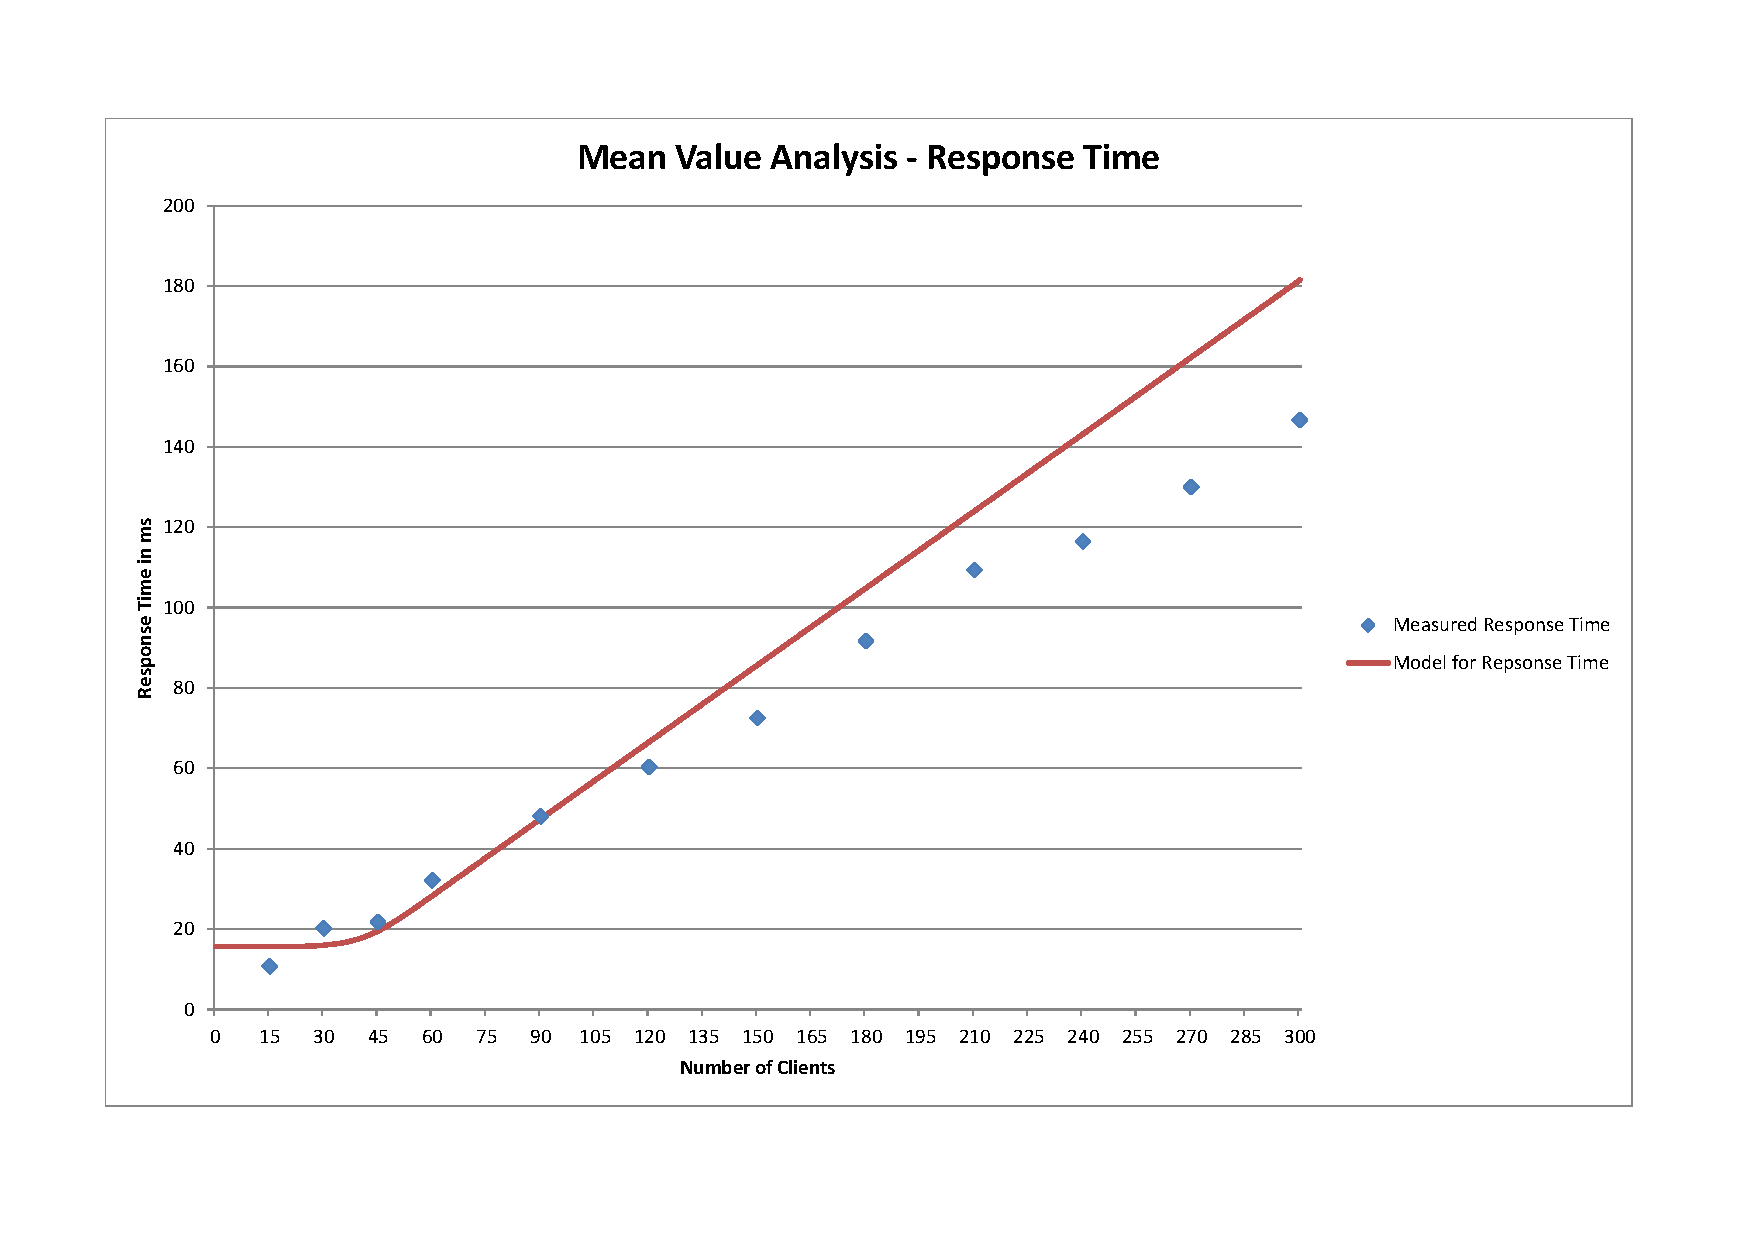
\includegraphics[scale=0.7, trim = 23mm 34mm 24mm 25mm, clip]{measurements_increase_load/rt_total.pdf}
  \end{center}
  \caption{mean value analysis, response time}
  \label{fig:rt_total}
\end{figure}

\begin{figure}[H]
	\begin{center}
    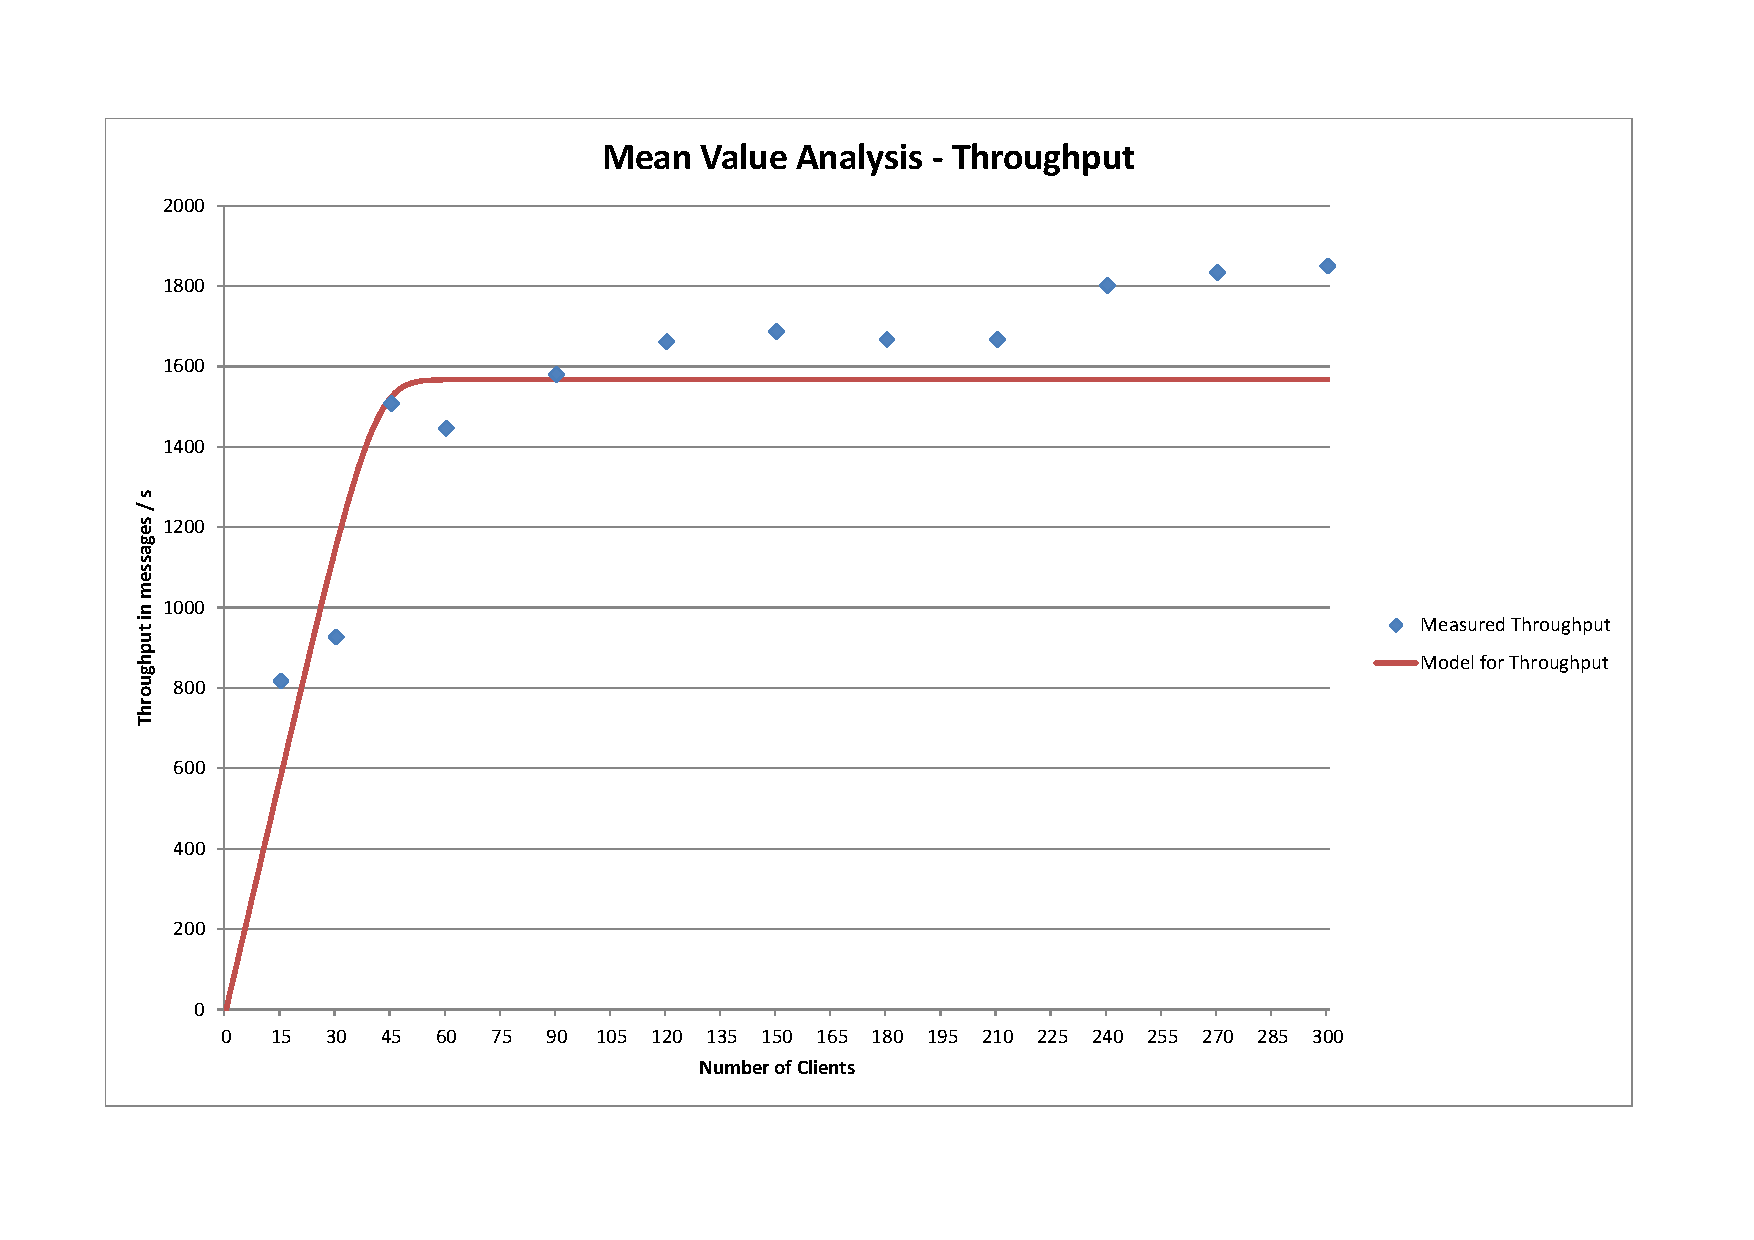
\includegraphics[scale=0.7, trim = 23mm 34mm 24mm 25mm, clip]{measurements_increase_load/tp_total.pdf}
  \end{center}
  \caption{mean value analysis, throughput}
  \label{fig:tp_total}
\end{figure}


\begin{figure}[H]
	\begin{center}
    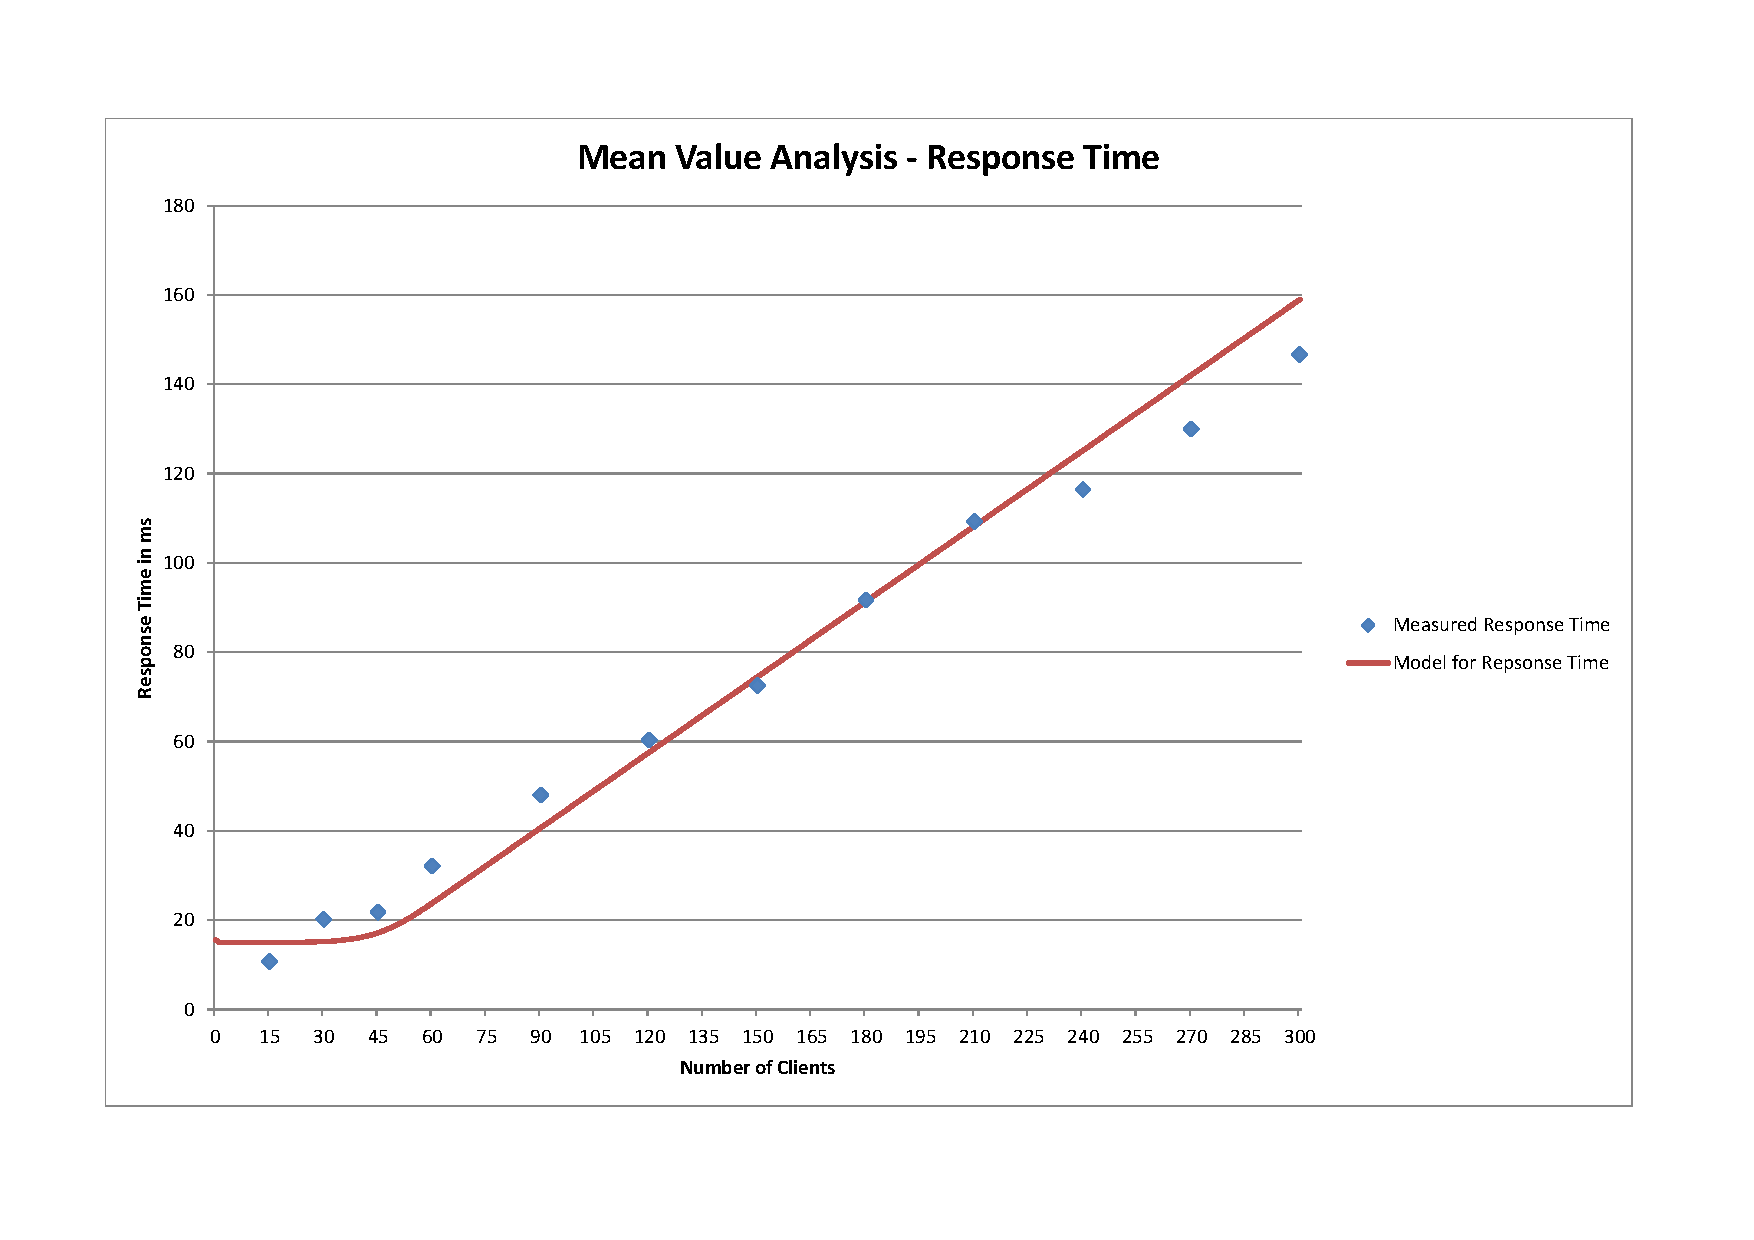
\includegraphics[scale=0.7, trim = 23mm 34mm 24mm 25mm, clip]{measurements_increase_load/rt_total_fixed.pdf}
  \end{center}
  \caption{mean value analysis, response time fixed}
  \label{fig:rt_total}
\end{figure}

\begin{figure}[H]
	\begin{center}
    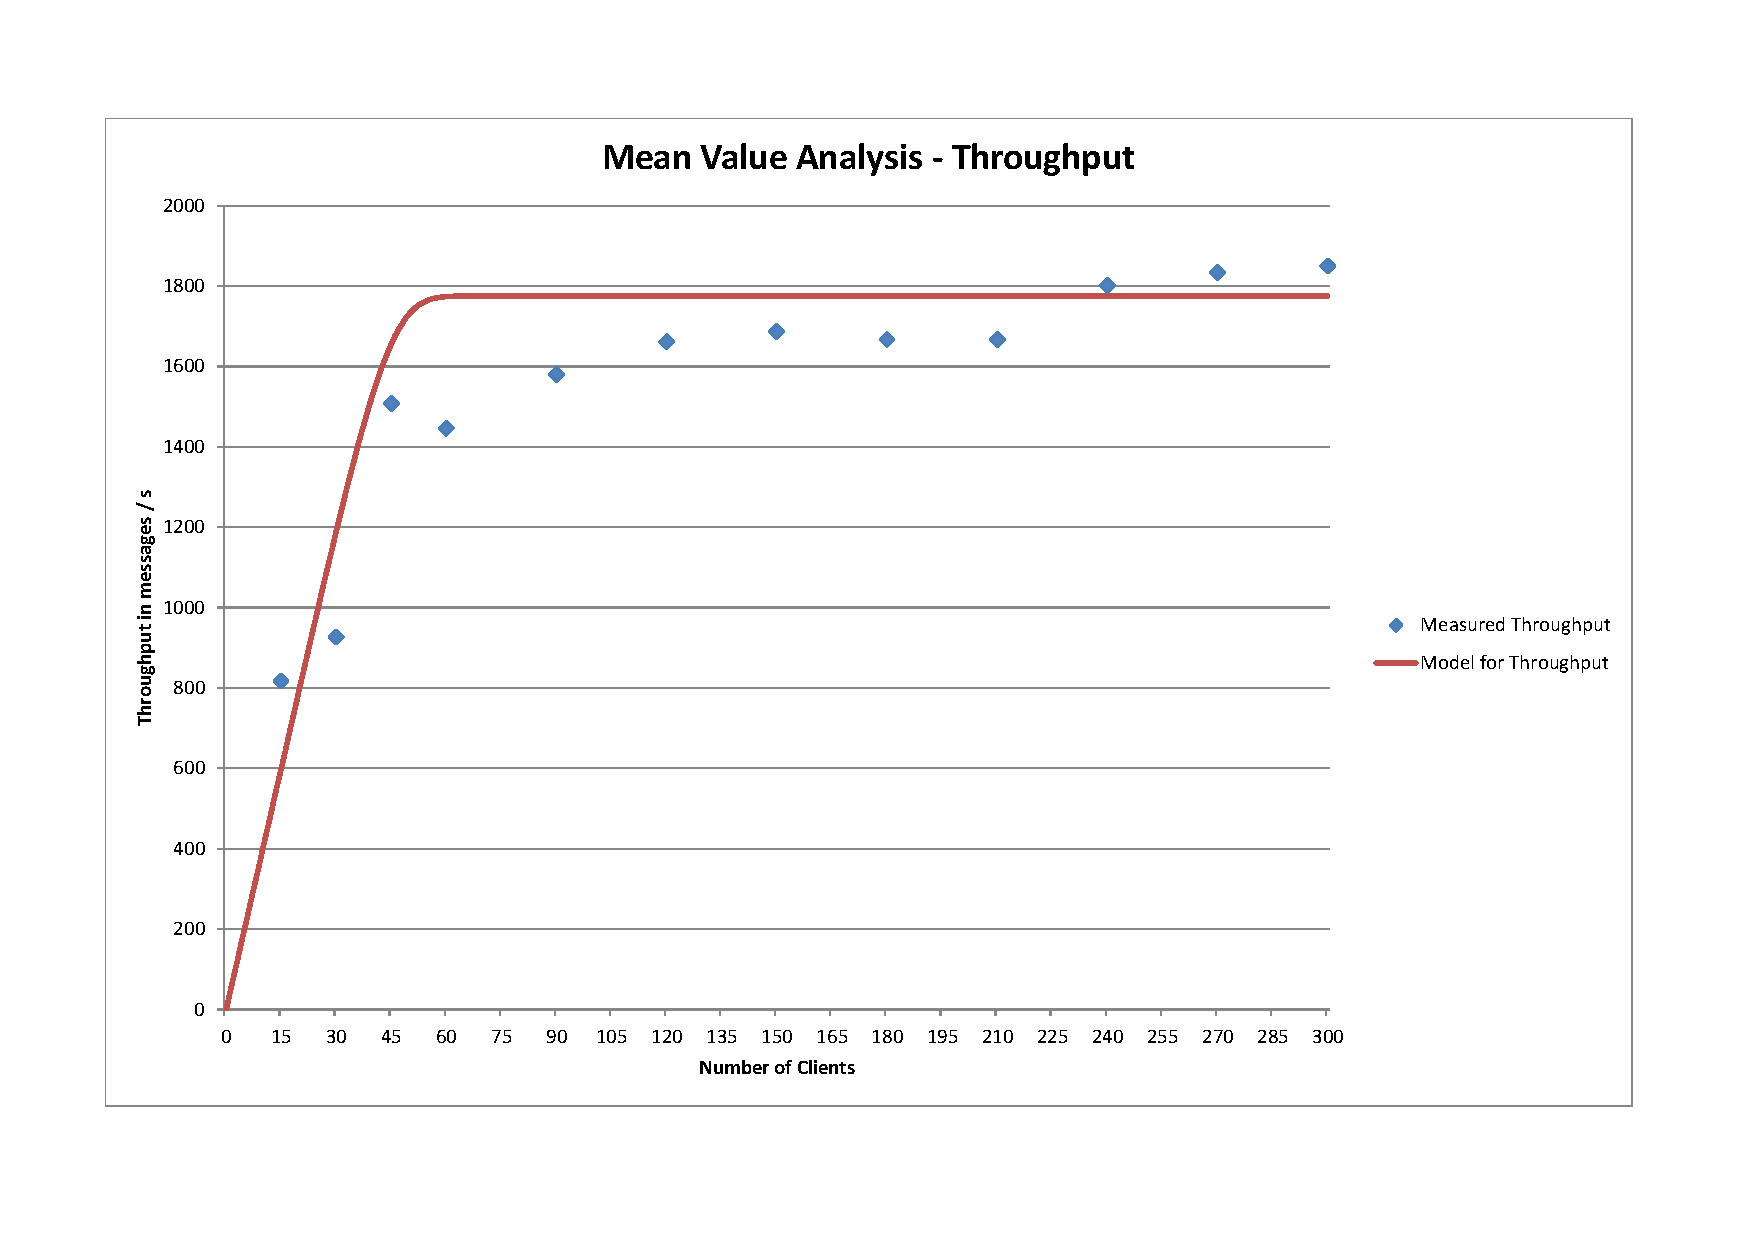
\includegraphics[scale=0.7, trim = 23mm 34mm 24mm 25mm, clip]{measurements_increase_load/tp_total_fixed.pdf}
  \end{center}
  \caption{mean value analysis, throughput fixed}
  \label{fig:tp_total}
\end{figure}

\end{landscape}



\subsubsection{Interpretation}

The first analysis without the adjusted service time for the database yielded not so good results for the response time. The mean value analysis for the response time seems pretty well. However, there seemed to be a additional constant of about 50ms where the response time of the model didn't match. It clearly can be observed that the measured response time and the modelled response time diverge, see figure \ref{fig:rt-total}. Also, the measured throughput is clearly higher then the modelled throughput, see figure \ref{fig:tp-total}. For those reasons, the mean service time of the database was adjusted and the fixed model was generated.\\

The analysis of the fixed model yields decent results, especially for the response time. The response time can be seen in figure \ref{fig:rt-total-fixed} and the throughput can be seen in figure \ref{fig:tp-total-fixed}.


\subsubsection{Possible Further Investigations}

As described in the simplified model description, the system could be modelled differently, by splitting up the database for sending and receiving into two separate parts. I think that this way, the model would be more accurate compared to the measured data. However, the trade-off between model complexity and best fit is always tricky, and I chose to stay with the slightly simplified model.








\end{document}









